%%%%%%%%%%%%%%%%%%%%%%%%%%%%%%%%%%%%%%%%%%%%%%%%%%%%%%%%%%%%%%%%%%%%%%%%%%%
%% This file is part of the book
%%
%% Algorithmic Graph Theory
%% http://code.google.com/p/graph-theory-algorithms-book/
%%
%% Copyright (C) 2009, 2010, 2011 Minh Van Nguyen <nguyenminh2@gmail.com>
%%
%% See the file COPYING for copying conditions.
%%%%%%%%%%%%%%%%%%%%%%%%%%%%%%%%%%%%%%%%%%%%%%%%%%%%%%%%%%%%%%%%%%%%%%%%%%%

\documentclass{article}

\usepackage{amsmath}
\usepackage{subfigure}
\usepackage{tikz}
\usetikzlibrary{external}
\tikzexternalize{Shannon-multigraphs}
\DeclareMathOperator*{\Sh}{Sh}  %% Shannon multigraphs

\begin{document}

\begin{figure}
%% Shannon multigraph Sh(2)
\subfigure[$\Sh(2)$]{
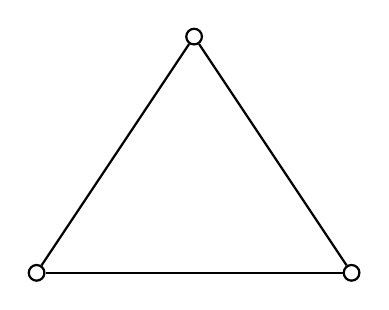
\begin{tikzpicture}
[nodeDecorate/.style={shape=circle,inner sep=2pt,draw,thick},%
  lineDecorate/.style={-,thick}]
%% nodes or vertices
\foreach \nodename/\x/\y in {a/-2/0, b/2/0, c/0/3} {
  \node (\nodename) at (\x,\y) [nodeDecorate] {};
}
%% edges or lines
\path
\foreach \startnode/\endnode in {a/b, b/c, c/a} {
  (\startnode) edge[lineDecorate] node {} (\endnode)
};
\end{tikzpicture}
}
\quad
%%
%% Shannon multigraph Sh(3)
\subfigure[$\Sh(3)$]{
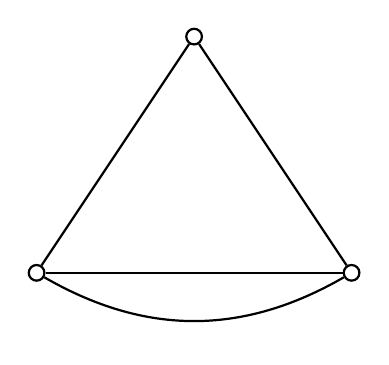
\begin{tikzpicture}
[nodeDecorate/.style={shape=circle,inner sep=2pt,draw,thick},%
  lineDecorate/.style={-,thick}]
%% nodes or vertices
\foreach \nodename/\x/\y in {a/-2/0, b/2/0, c/0/3} {
  \node (\nodename) at (\x,\y) [nodeDecorate] {};
}
%% edges or lines
\path
\foreach \startnode/\endnode in {a/b, b/c, c/a} {
  (\startnode) edge[lineDecorate] node {} (\endnode)
}
(a) edge[lineDecorate,bend right] node {} (b);
\end{tikzpicture}
}
\quad
%%
%% Shannon multigraph Sh(4)
\subfigure[$\Sh(4)$]{
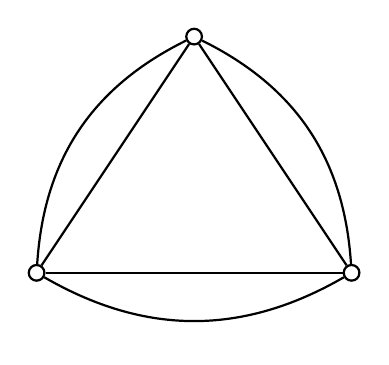
\begin{tikzpicture}
[nodeDecorate/.style={shape=circle,inner sep=2pt,draw,thick},%
  lineDecorate/.style={-,thick}]
%% nodes or vertices
\foreach \nodename/\x/\y in {a/-2/0, b/2/0, c/0/3} {
  \node (\nodename) at (\x,\y) [nodeDecorate] {};
}
%% edges or lines
\path
\foreach \startnode/\endnode in {a/b, b/c, c/a} {
  (\startnode) edge[lineDecorate] node {} (\endnode)
  (\startnode) edge[lineDecorate,bend right] node {} (\endnode)
};
\end{tikzpicture}
}
%%
%% Shannon multigraph Sh(5)
\subfigure[$\Sh(5)$]{
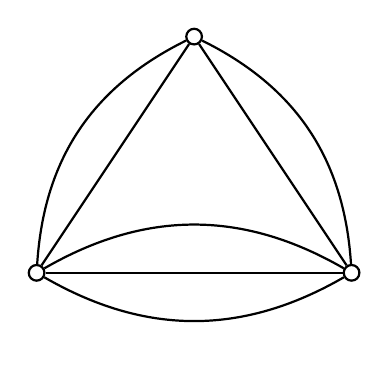
\begin{tikzpicture}
[nodeDecorate/.style={shape=circle,inner sep=2pt,draw,thick},%
  lineDecorate/.style={-,thick}]
%% nodes or vertices
\foreach \nodename/\x/\y in {a/-2/0, b/2/0, c/0/3} {
  \node (\nodename) at (\x,\y) [nodeDecorate] {};
}
%% edges or lines
\path
\foreach \startnode/\endnode in {a/b, b/c, c/a} {
  (\startnode) edge[lineDecorate] node {} (\endnode)
  (\startnode) edge[lineDecorate,bend right] node {} (\endnode)
}
(a) edge[lineDecorate,bend left] node {} (b);
\end{tikzpicture}
}
\quad
%%
%% Shannon multigraph Sh(6)
\subfigure[$\Sh(6)$]{
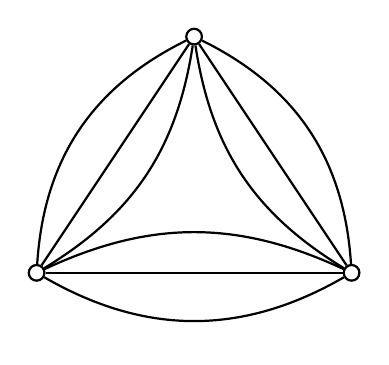
\begin{tikzpicture}
[nodeDecorate/.style={shape=circle,inner sep=2pt,draw,thick},%
  lineDecorate/.style={-,thick}]
%% nodes or vertices
\foreach \nodename/\x/\y in {a/-2/0, b/2/0, c/0/3} {
  \node (\nodename) at (\x,\y) [nodeDecorate] {};
}
%% edges or lines
\path
\foreach \startnode/\endnode in {a/b, b/c, c/a} {
  (\startnode) edge[lineDecorate] node {} (\endnode)
  (\startnode) edge[lineDecorate,bend right] node {} (\endnode)
  (\startnode) edge[lineDecorate,bend left=25] node {} (\endnode)
};
\end{tikzpicture}
}
\quad
%%
%% Shannon multigraph Sh(7)
\subfigure[$\Sh(7)$]{
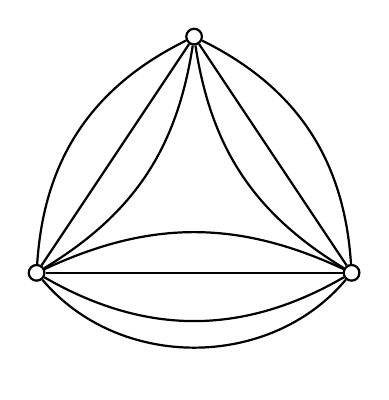
\begin{tikzpicture}
[nodeDecorate/.style={shape=circle,inner sep=2pt,draw,thick},%
  lineDecorate/.style={-,thick}]
%% nodes or vertices
\foreach \nodename/\x/\y in {a/-2/0, b/2/0, c/0/3} {
  \node (\nodename) at (\x,\y) [nodeDecorate] {};
}
%% edges or lines
\path
\foreach \startnode/\endnode in {a/b, b/c, c/a} {
  (\startnode) edge[lineDecorate] node {} (\endnode)
  (\startnode) edge[lineDecorate,bend right] node {} (\endnode)
  (\startnode) edge[lineDecorate,bend left=25] node {} (\endnode)
}
(a) edge[lineDecorate,bend right=50] node {} (b);
\end{tikzpicture}
}
\end{figure}

\end{document}
